\chapter*{Introduction}
\addcontentsline{toc}{chapter}{Introduction}
%\textbf{~5 pages}

% % ICI on touche pas les sections et on ne fait pas de sous section
% % La structure est standard

% In this section, you introduce your works, your vision, and why they are relevant. The goal of this section is to present, if possible,  the \textit{narrative} of your Master degree.




%\section*{Drone technologies}

Drones, or unmanned aerial vehicles (UAVs), have been around since the early 1900s. Drones can range from the size of airplanes to the size of bumblebees (Figure \ref{fig:airpollution}). Originally used for military operations, they became more widely used after about 2010 when electronic technology got smaller, cheaper and more efficient, prices on cameras and sensors dropped, and battery power improved \cite{xiang_xia_zhang_2020}\cite{overview_uavsensors}. Where once scientists could only observe earth from above by using manned aircraft or satellites, today they are expanding, developing and refining their research thanks to drones \cite{sørensen_jacobsen_hansen_2017} \cite{metrology_survey}\cite{xiang_xia_zhang_2020}.

\begin{marginfigure}%[!h]
      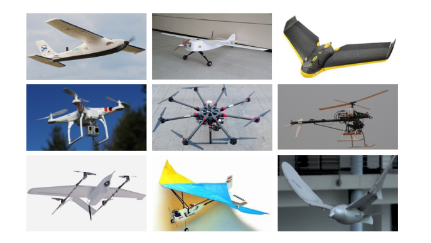
\includegraphics[width=6cm, center]{images/intro/mini_uavs.png}
      \caption{Examples of mini-UAVs used for remote sensing, from \cite{xiang_xia_zhang_2020}.} 
      \label{fig:mini_uavs}
\end{marginfigure}

% \begin{marginfigure}%[!h]
%       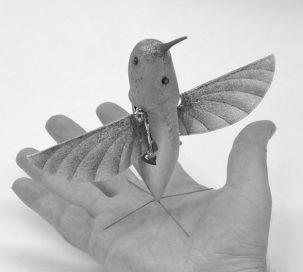
\includegraphics[width=5cm, center]{images/intro/nano_hummingbird_bw.jpg}
%       \caption{The Nano Hummingbird drone is used for surveillance by DARPA.} 
%       \label{fig:hummingbird}
% \end{marginfigure}

\begin{marginfigure}%[h]
    \raggedright 
    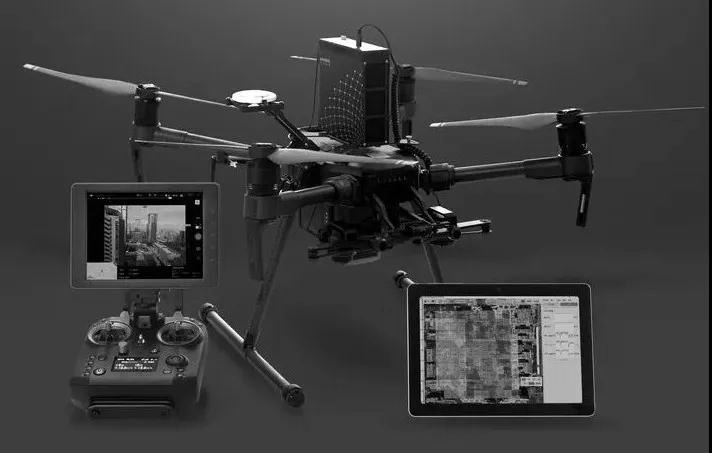
\includegraphics[width=5cm]{images/stage_graphs/environment_results/air_monitoring_drone_bw.jpg}
    \caption{DJI Matrice 200 with onboard gas detector (from DJI's website, 2021)}
    \label{fig:airpollution}
\end{marginfigure}    

Depending on their mission, drones are equipped with different payloads or equipment (Figure \ref{fig:airpollution}). Digital cameras can identify plants and animals, and help create 3-D maps.  Thermal cameras detect heat from living creatures like animals or stressed plants, as well as from water \cite{metrology_survey}. Hyperspectral imaging identifies features of plants and water through measuring reflected light and can interpret a wider range of wavelengths than the human eye can see. LiDAR, which measures how long it takes for an emitted pulse of light to reach a target and return to the sensor, can be used to calculate the distance to an object and its height, which is used for 3-D maps \cite{metrology_survey}. With this range of sensors, scientists and practitioners can choose from a range of options to expand their research. 

We see great growth in mobile mapping research, that is “the acquisition of spatiotemporal phenomena by
using a mobile multi-sensor platform” \cite{mobile_mapping}. This field of research includes remote sensing \cite{remote_sensing} the acquisition of information about an object or phenomenon without making physical contact with the object, as well as various contact-based techniques \cite{sensor_placement_uav} for the acquisition of information in direct contact with the object.

\begin{marginfigure}%[!h]
  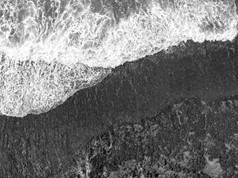
\includegraphics[width=5cm, center]{images/intro/coastal_bw.jpg}
  \caption{Drone picture of coastline after a storm.} 
  \label{fig:coastal}
\end{marginfigure}

Inspection and Data Gathering is an area of scientific study that is gradually adopting drones. For instance, the Sea Level and Coastal Changes group at MARUM (University of Bremen) \cite{scientific_research} studies coastal erosion, mangrove communities as well as the distribution of corals and the death of shallow corals. Prior to drones, the typical thing to do is to put a GPS on your backpack and walk along the beach to actually measure points on the beach. Coastal areas change rapidly for example, before and after a storm (Figure \ref{fig:coastal}). Instead, The drones take many pictures at short intervals, and repeat flights at short intervals can show differences in conditions. A drone can cover the same area in less time and get much higher resolution pictures. This demonstrates that these tools are an ideal integration in a data gathering toolkits of researchers and practitioners. As a result, the industrial usage of drones is growing steadily. 


% The future of drone flight can be explored through the lens of dedicated markets \cite{}. the 6th NeTWork alongside (Figure \ref{fig:6thnetwork}). Recent developments in the European Airspace (November 2020) have led to various drone consortiums, such as  This new airspace allows for drones for business applications. An air channel for drone transport of supplies. There is also a nascent market for Inspections and Data gathering.

% \begin{figure*}[!h]
%   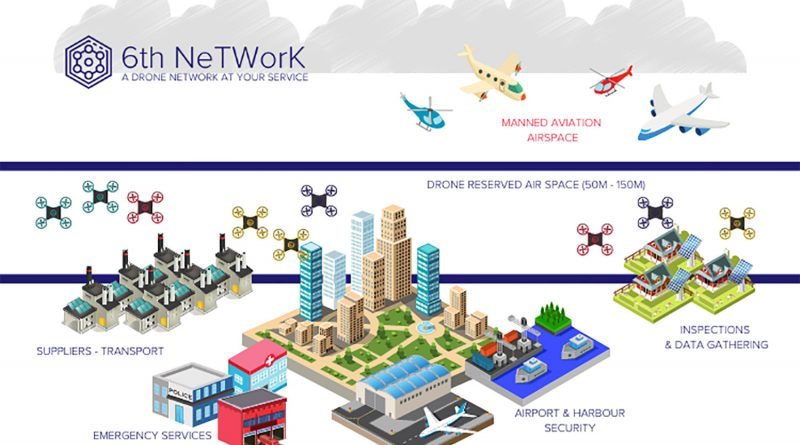
\includegraphics[width=13cm, center]{images/6th-network-drone-as-a-service.jpg}
%   \caption{Drone markets opened for business applications} 
%   \label{fig:6thnetwork}
% \end{figure*}
% Further investigation demonstrates a host of services that employ drones. According to [consulting] \cite{}, drones are applicable in areas as diverse as surveillance and monitoring, inventory management, search and rescue, or in the entertainment industry.  

% % [examples to illustrate this point: 
% % \begin{itemize}
% % \item Research on Drone Monitoring: air pollution consortium, pollution abatement
% % \item Military Applications and Drone Racing leading the way for emergency services
% % \item Public services: firestations, train tracks, civil engineering, even insurance companies
% % \end{itemize}
% % ].


% In recent years there have been significant advancements in this
% research field. The current use of swarms is generally based on custom, centralized solutions, in environments with reliable communication \cite{buzz_swarm_stack}.
% % Most small drones are powered by lithium-polymer batteries, while larger ones may use airplane engines. Many drones are made of carbon fiber making them light and easy to land without disturbing the environment. 

% The French Security Authority on Civil Aviation (DGAC) requires that drones remain within the operator’s line of sight; larger drones that fly longer distances must obtain more involved licenses that allow them to fly outside of the line of sight \cite{dsac_2021}. As a result, UAV swarms rarely leave the controlled and safe environment of laboratories, and when they do it is for short-duration experiments. 

%\section*{Challenges for Specialised Drones}

All in all, applications for drones are crossing boundaries of science and industry, with everything from aerial photography to package delivery to disaster management benefiting from the technology. But before they become commonplace, there are challenges to be solved to make them reliable and safe. 

% \begin{marginfigure}%[!h]
%   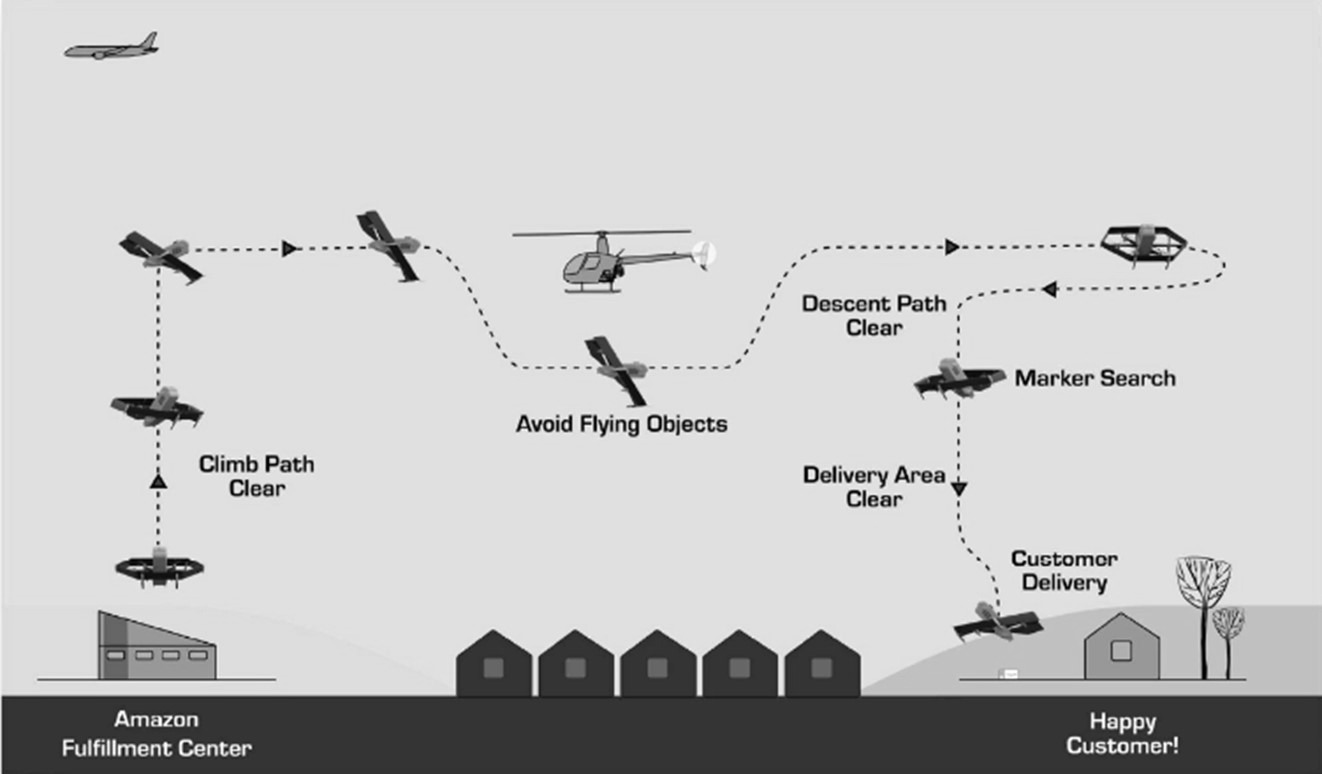
\includegraphics[width=5cm, center]{images/intro/amazon_deployment_bw.jpg}
%   \caption{Deployment process from Amazon Station \cite{}} 
%   \label{fig:amazon_deployment}
% \end{marginfigure}

%  As an operation scales in complexity, it requires exponentially more resources. Equipment, training and safeguards are vital. 

Drones are usually flown with a controller on the ground, and some form of wireless communication (usually radio signals) between the operator and the drone  \cite{xiang_xia_zhang_2020}. Since the remote pilot focuses on navigational aspects, it restricts the range of flights of a single operator. A challenge to drone flight is the amount of human involvement. \cite{zhou_gheisari_2021} looks at the capacity of the research team collecting data. Five provided information regarding the human involvement in their experiments; four of which are damage assessment. Pratt et al. \cite{pratt_operator1} (2008) included four members in their UAS operation crew: a pilot, a safety manager, a mission specialist and a tether manager. Kruijff et al. (2012) \cite{Kruijff_operator2} applied the same team structure as Pratt et al. (2008), less the tether manager. Murphy et al. (2008) \cite{murphy_operator3} discussed extensively the responsibility of each team member in a UAS flight and recommended a crew of three: a pilot, a mission specialist and a flight director.

In developing complex functionalities, the operator is focused on remote piloting, or on manning the ground station. In so doing, the operation requires further automation in order to give more flexibility to the operator, and in their amount of involvement. 

A window of opportunity for the quality and application possibilities of industrial drones is the built-in sensor technology \cite{scientific_research}. Sometimes referred to as smart drones, additional monitoring systems can be installed between a drone's flight control and smart sensors \cite{uav_components}. Ideally, this allows for more efficient motors, better on board processors and software, more accurate sensors, as seen in Figure \ref{fig:drone_gens}, built-in safeguards, networked together to enable coordination, collaboration and real time data delivery, etc. 

\begin{figure*}[!h]
  \raggedright
  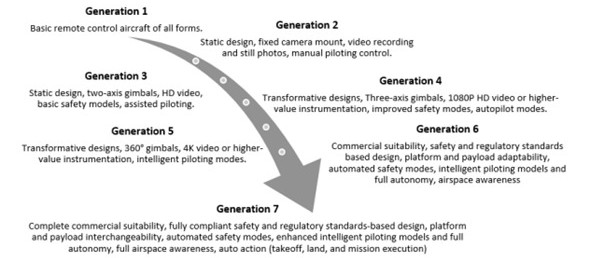
\includegraphics[width=11.5cm]{images/intro/gen_evolution_bw.jpg}
  \caption{Generations of drone technology.} 
  \label{fig:drone_gens}
\end{figure*}

There are challenges to implementing smart sensors, which is the length and difficulty of the development process. For instance, collision avoidance is generally recognised as a complex process \cite{landing_challenges}\cite{autonomy_survey}. This complexity can be attributed to the many different variables that factor in based on the applications in which this technology is used. Collision detection requires regular input of altitude, which is usually transmitted by an onboard range sensor. Additionally, with a view of obstacle, the drone can estimate. This is delegated to a camera or radio frequency sensor. Furthermore, algorithms would be required to monitor a obstacles relative to the moving drone, or detect if noise is an obstacle, which is solved with finer state estimation techniques \cite{px4_landing}. 

\section{Problem Statement}

In this thesis, I examine how smart systems benefit UAVs, and the tasks in which they operate. The problem I address is to understand the tradeoffs of certain smart systems over others in assisting UAV functionality.
% problem_statement}

What environments, and tools, can we put at disposition to accelerate the development of specialised functionalities using drone equipment? What functionalities are ideally developed in a research setting, as opposed to an industrial one? Are there any functionalities which require specific technological integrations? Should these functionalities be developed before flight, or during flight? This last distinction is the basis for two separate approaches: a dedicated test-and-demonstrate environment as opposed to a ground station.

%\section*{Approaches}


% \begin{marginfigure}%
%   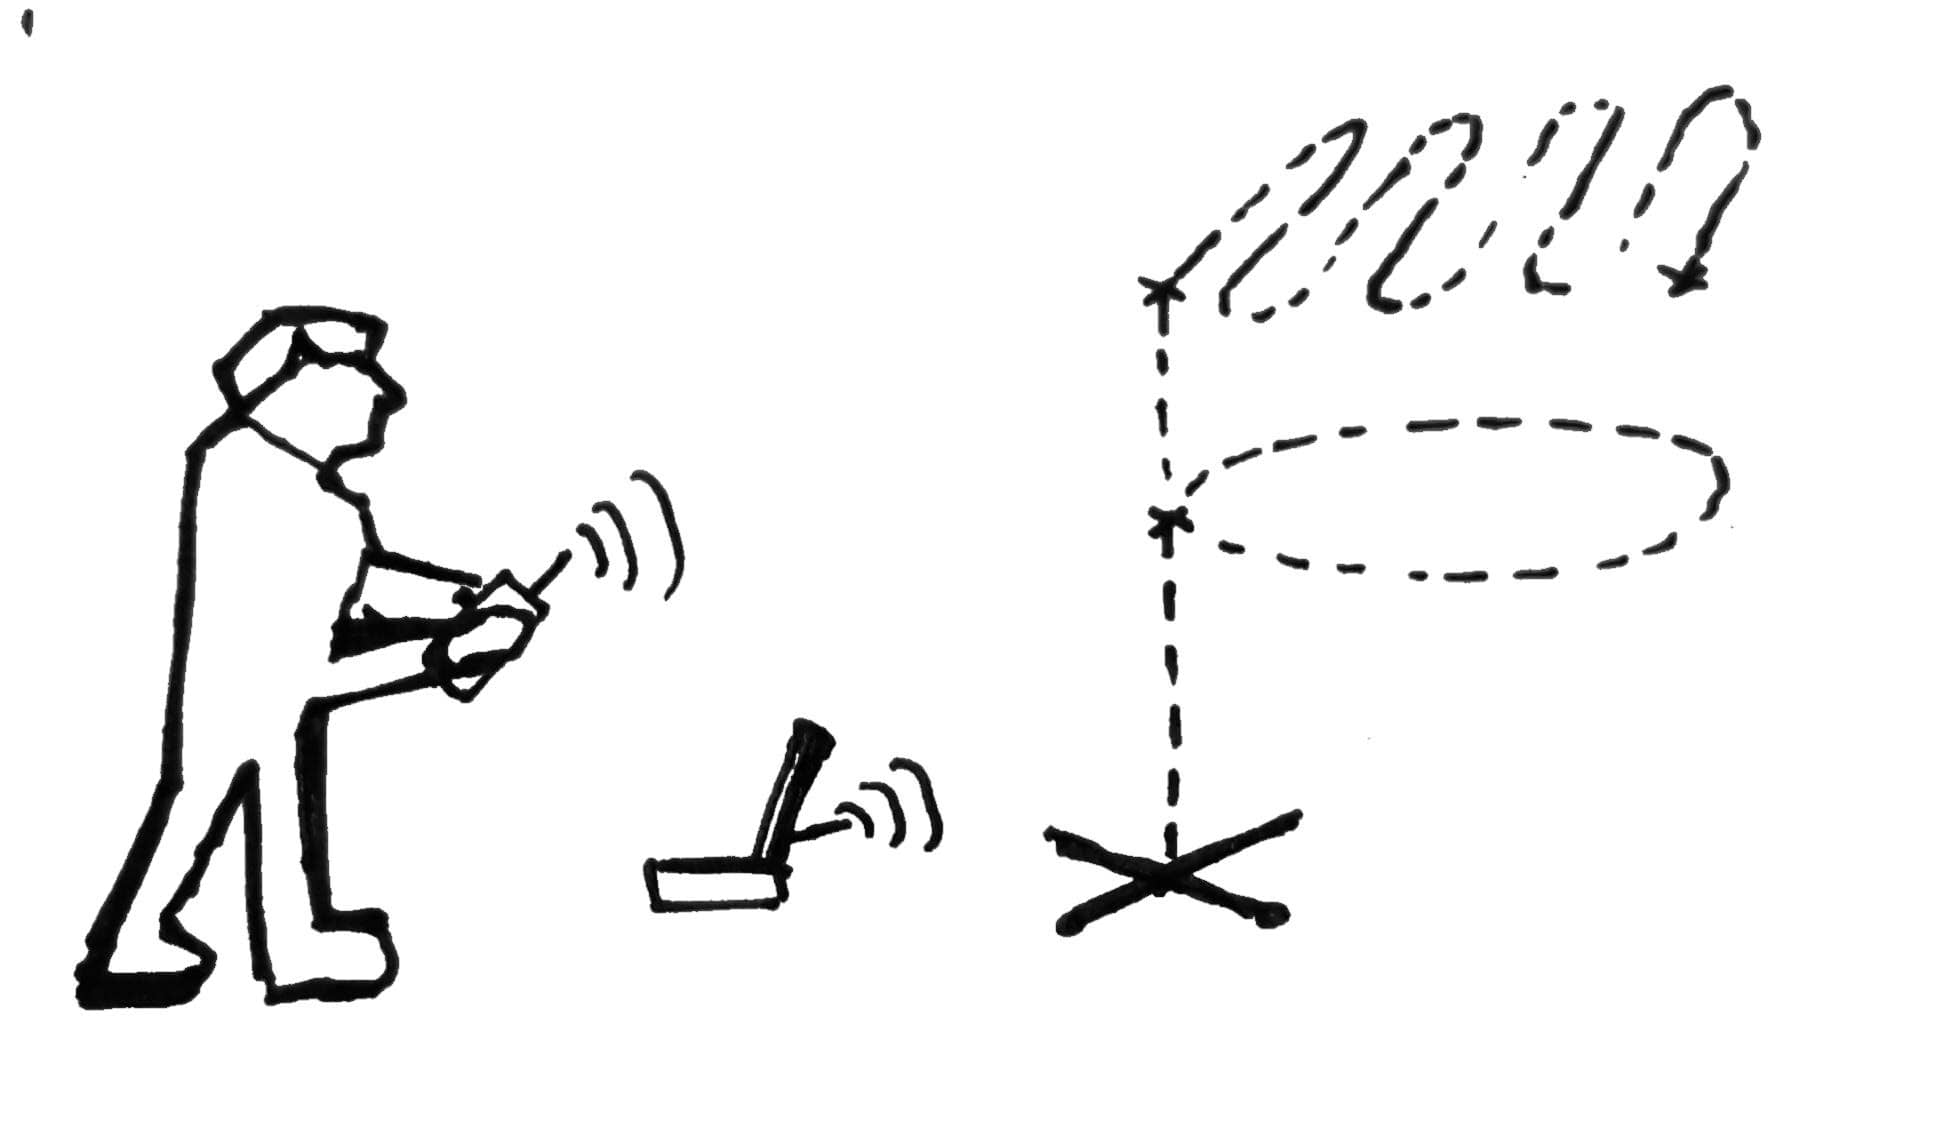
\includegraphics[width=5cm]{images/intro/concept_groundstation.jpg}
%   \caption{A ground station.}
%   \label{fig:hand_piloting_intro}
% \end{marginfigure}
\textbf{The first approach explores the potential of distributed systems to assist task development upon UAVs.
}
% \textbf{approachA_question}}
\begin{marginfigure}%
  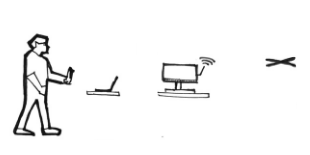
\includegraphics[width=5cm]{images/intro/step2_diagram.png}
  \caption{A dedicated test-and-demonstrate environment.}
  \label{fig:approachA}
\end{marginfigure}
% approachA_goal}
In our first approach, we examine distributed systems, whereas multiple systems coordinate to assist, and simplify tasks during development and demonstration. This is a systemic approach that aims to interconnect the available systems. For instance, smart sensors can control a drone’s navigation path and monitor its flight. The operator's interactions can be guided by computer vision systems along with object detection and collision avoidance programs. New forms of artificial intelligence or algorithms can make them even more adaptable. We explore the ways in which distributed systems can spare the practitioner from repetitive and time-consuming tasks.

% \textbf{approachB_question}}
\textbf{The second approach explores the potential of  onboard systems to assist the real-world deployment of UAVs.}
\begin{marginfigure}%
  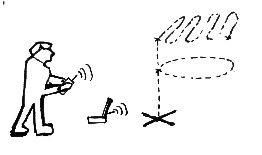
\includegraphics[width=4cm]{images/intro/outputonlinejpgtools.jpg}
  \caption{An environment for outdoor deployments.}
  \label{fig:approachB}
\end{marginfigure}
% approachB_goal}
In a second approach, we look more closely at the interplay between smart systems, and the real-world deployment of a UAV. We investigate how a drone's design aids to gather multi-faceted data. Data acquisition systems offer an opportunity to manage the data collection process. Specialised navigation tasks offer other means of automating the data collection process. The drone operator can examine the data gathered in real time, and becomes involved as a data interpreter. We explore the ways in which onboard systems can aid with the practitioner’s task.


\section{Research Domains}

This thesis is associated with three major fields of work: swarm engineering, human drone interfaces and mobile sensing. These fields take inspiration from a variety of other fields. Figure \ref{fig:research_domains} shows several domains that are explored in this thesis.


% \smartdiagram[bubble diagram]{
%         \textbf{Drone}\\
%         \textbf{Automation},
%         \textbf{HCI}
%         \textbf{Swarm}\\
%         \textbf{Engineering},
%         \textbf{Swarm}\\
%         \textbf{Engineering},
%         \textbf{Mixed}\\
%         \textbf{Reality Interfaces},
%         \textbf{Computer}\\
%         \textbf{Vision},
%         \textbf{Drone System}\\ 
%         \textbf{Design},
%         \textbf{Onboard Data}\\ 
%         \textbf{Acquisition}
%     }

\begin{figure*}[!h]
  \raggedright
  \includegraphics[width=11cm]{images/intro/research_domains.png}
  \caption{Research domains explored in this thesis.} 
  \label{fig:research_domains}
\end{figure*}

%swarm_engineering_field
According to \citetitle{swarm_review} \cite{swarm_review}, swarm robotics is an approach to collective robotics that takes inspiration from the self-organized behaviors of social animals. Through simple rules and local interactions, swarm robotics aims for robust, scalable and flexible collective behaviors for the coordination of large numbers of robots. In contrast, the term swarm engineering \cite{swarm_engineering} describes the design of predictable, controllable robot swarms with well-defined goals and the ability to function under certain conditions. Swarm engineering focuses mainly on concepts that could be relevant for real-world applications, therefore shifting swarm robotics to engineering applications. 

%hdi_field}
In \citetitle{tezza_andujar_2019} (\citeyear{tezza_andujar_2019}), \citename{tezza_andujar_2019}{author} define Human-Drone Interaction (HDI) as a field of research that consists of understanding, designing and evaluating drone systems for use by humans, and in contact with humans. This field is similar to human-robot interaction (HRI), however, a drone’s unique characteristic to freely fly in a 3D space, and unprecedented shape makes human-drone interaction a research topic of its own. Researchers develop control modalities and better understand means of communicating with a drone.

%mobile_mapping_field}
We see great growth in mobile mapping research, that is “the acquisition of spatiotemporal phenomena by using a mobile multi-sensor platform” \cite{mobile_mapping}. The UAV is a platform that greatly simplifies research. One such field remote sensing, the acquisition of information about an object or phenomenon without making physical contact with the object \cite{remote_sensing}. Recently, UAVs have enabled research towards contact sensing, for the acquisition of information in direct contact with the object \cite{sensor_placement_uav}, on a platform that serves for optimal sensor placement \cite{sensor_placement_uav} \cite{stewart_chang_sudarchan_becker_huang_2016}.

% Drone swarms are ideal for missions involving large areas and a high level of detail. Other applications can involve heavy parts moving by multiple drones, drone writing in the sky or other drone shows, etc. AI drones used in automated infrastructure inspections not only perform safe and efficient surveillance but, thanks to their Machine Learning capabilities, they are also able to analyse the large volume of images to identify patterns and/or map the images to detect anomalies in data. Machine Learning is the key to unleash the drone inspection’s true potential.

% \section{Research Approaches}

% The following Approaches are investigated in this thesis.

% \smartdiagram[bubble diagram]{
%         \textbf{Drone}\\
%         \textbf{Automation},
%         \textbf{Multi-robot}\\
%         \textbf{infrastructure},
%         \textbf{Task}\\
%         \textbf{Management},
%         \textbf{Real-time}\\
%         \textbf{Pilot Pipelines},
%         % \textbf{System Design}\\
%         % \textbf{From Direct Input},
%         % \textbf{Sensor}\\ 
%         % \textbf{Characterisation}
%     }

% \section{Research Methods}

% \smartdiagram[bubble diagram]{
%         \textbf{Drone}\\
%         \textbf{Automation},
%         \textbf{Testbed}\\
%         \textbf{Evaluation},
%         % \textbf{}\\
%         % \textbf{Management},
%         \textbf{Controller}\\
%         \textbf{Response Times},
%         \textbf{System Design}\\
%         \textbf{From Direct Input},
%         \textbf{Sensor}\\ 
%         \textbf{Characterisation}
%     }

\section{Contributions}



This list of contributions outlines each project in its respective field and an overview of the approach used to evaluate it.

\textbf{\nameref{c1}}



\textit{A Multi-Robot Management Layer}

% {multi_robot_why}
We motivate a smarter ecosystem for task development upon drones by beginning with the infrastructure for new technologies and for prototyping functionalities. A centralised swarm framework serves to set up flight performance monitoring systems, a fundamental asset to the development of robots and multi-robot groups \cite{gcs_validation}. 
% {stability_test_evaluation}
A hover stability test is a good measure of system performance since it requires quick readjustments of the drone to counter natural disturbances during hovering. In \cite{experimental_tuning}, \citename{experimental_tuning}{author} determine the performance of their flight controller by comparing the attitude of the drone in relation to the demanded null value of angular rotations. In this experiment, two drones are required to hover at an input setpoint with minimal error. The error over time is compared for the drones to better understand flight stability.


\textit{A High Level Interface}

% {high_level_interface_why}
A high level interface is an abstraction layer for development activities. In order to simplify task development, and align with the thesis goals, we develop a framework for high level interaction between the operator and the functionalities of the testbed.
% {high_level_interface_demonstration}
A drone choreography is designed as a live demonstration of the Testbed's functionality. The experiment data is accessible publicly \cite{choreography_data}.

\begin{marginfigure}%[h]
    \raggedright
    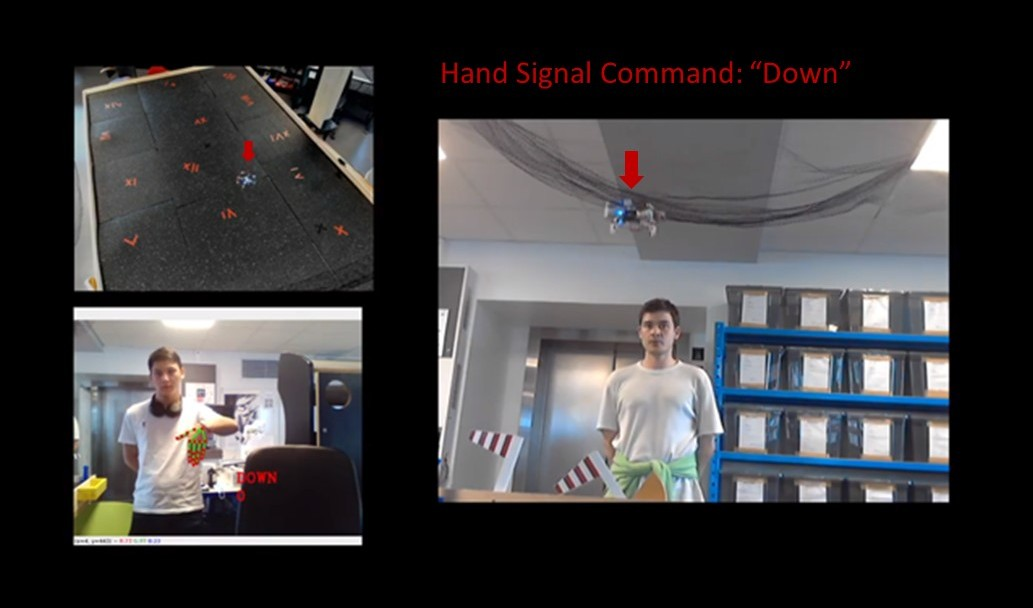
\includegraphics[width=5cm]{images/Signal_Mode.JPG}
    %\includegraphics[width=7.6cm]{images//DSCF0871.jpg}
    \caption{Presentation video \cite{piloting_video} of the Gesture Recognition Pipeline}
\end{marginfigure}
\textbf{\nameref{c2}}

\textbf{A Gesture Controller for UAV Piloting}

% gesture_interface_why}
As of \citedate{tezza_andujar_2019}, multiple gesture interfaces have been developed for UAVs \cite{liu_szirányi_2021} \cite{gesture_interface}, but are lacking in drone piloting. Realtime interfaces for drone piloting are discouraged \cite{tezza_andujar_2019} due to high latency and low control precision compared to other drone control modalities. As of \citedate{crazyflie_research}, the literature utilizing the Crazyflie nanodrone does not include realtime streaming commands \cite{crazyflie_research}. 

% gesture_interface_overview}
We put in place a demonstration for flight piloting in real-time using the developed gesture interface. 
We present the workflow of real-time gesture piloting pipeline and we evaluate it in terms of:
\begin{itemize}
    \item System response time
    \item Accuracy of gesture recognition
\end{itemize}

\textit{Effective Gesture Recognition} \hspace {0.5cm} In order to evaluate gesture recognition performance, \cite{bolin_crawford_macke_hoffman_beckmann_sen_2017} evaluates the false positive and negative rates of the pose detection by manually identifying both the incorrectly recognised gestures, and the unrecognised gestures. Similarly, we identify the false positive and negative rates of the pose detection.%gesture_recognition_evaluation}


\textit{A Pipeline with minimal Response Time} \hspace{0.5cm} The system response time was verified by applying a series of rapid maneuvers to register any significant delays between the pilot’s commands and their execution by the flight control system. \citename{experimental_tuning}{author} \cite{experimental_tuning} choose to modify the drone’s angle in a specified direction. This choice is arbitrary and the changes in velocity are used in this case.The input was a demanded velocity in a specified direction. The input was changed randomly by the operator with hand movements. The output was a delay of the velocity change in the drone. Finally, a system response time is determined by averaging the response delays over the experiment. %response_time_evaluation}

\begin{marginfigure}%[!h]
    \raggedright
    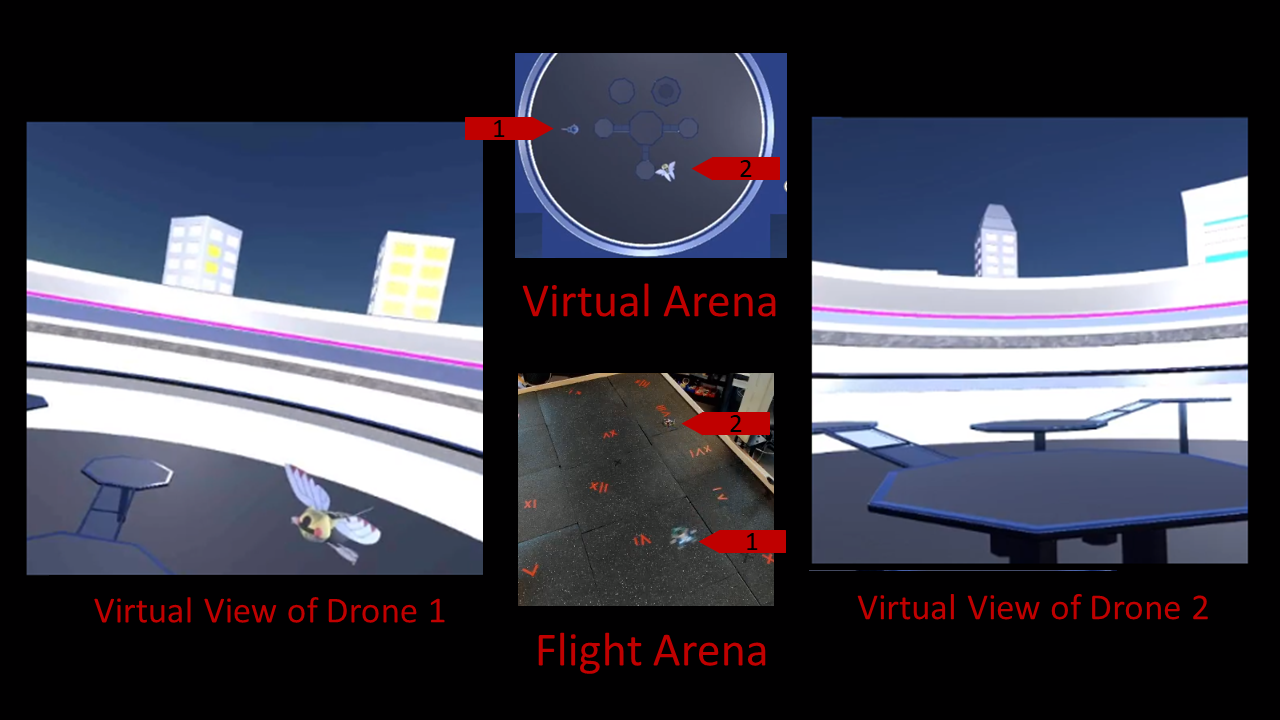
\includegraphics[width=5cm]{images/xr_pres.png}
    \caption{Video feeds of Mixed Reality Setup. The setup is maintained as a Github repository \cite{mixedreality_github} and a presentation video is available \cite{mixedreality_video}}
\end{marginfigure}

\textbf{A Mixed Reality Setup for Drone Development}

% mixed_reality_why}
The first objective of the simulated environment is to serve as a graphical interface in order to develop tasks otherwise too difficult to deploy. The priority of the virtual reality is therefore set on rendering capabilities, and the ability to obtain camera streams from this environment. 
% mixed_reality_overview}
We set up a virtual interface between real and virtual objects in real time. This MR simulation consists of a network interface between a robotics backend (ROS) and virtual environments (Unity3D). Similarly to \cite{mr_planetary}, the pipeline is then evaluated in terms of communication latency for two separate scenarios.
\begin{itemize}
    \item when transmitting parameters into the simulated environment
    \item when transmitting parameters to the robotics backend.
\end{itemize}

\textit{The latency of data transmission into the virtual setup}

% mixed_reality_evaluation1}
This latency is evaluated by determining the time-delay between the detection of drone poses from the robotics backend and the time they are received in the virtual setup. This approach is also taken in \cite{mr_planetary}, who observe that on average a 400 ms time delay occurred in their MR simulation.

\textit{The latency of data transmission out of the virtual setup}

% mixed_reality_evaluation2}
This latency is evaluated by determining the time-delay between the detection of an event from the virtual setup, and the time that they cause a state change in the drone’s task manager. This approach deviates slightly from \cite{mr_planetary}, who measure the moment the information is displayed on their graphical interface. Both approaches measure the response time before the event-data has its intended effect.

\textit{\textbf{\nameref{c3}}}

% {drone_design_why}

\begin{marginfigure}%[h]
    \raggedright. 
    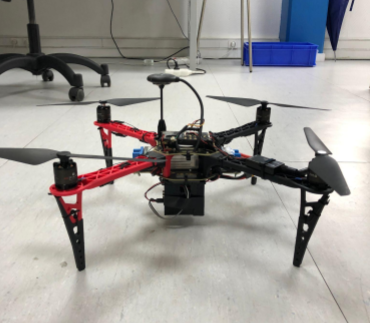
\includegraphics[width=5cm]{images/stage_system/drone_setup.png}
    \caption{Data Acquisition System setup. }
    \label{fig:damping_intro} 
\end{marginfigure}    


\textit{Optimal Payload Shock Absorption for Optimised Payload Transport}

% vibration_test_evaluation}
We test the vibration sensitivity of the payload to remove any parasitic vibrations. We compare the shock absorption of two payloads subject to different amounts of damping material. This is done by developing a vibration profile as direct input from two accelerometers during drone flight and increasing the volume of damping material. 

%FIELD SCAN
\begin{marginfigure}%[!h]
    \raggedright
    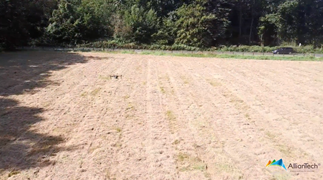
\includegraphics[width=5cm]{images/stage_graphs/environment_results/Flight_Drone.png}
    \caption{Field Scans}
    \label{fig:fieldscanpic}
\end{marginfigure}

\textit{Monitoring Environment Conditions with a Drone Fieldscan Solution}

% field_scan_evaluation}
We develop a drone solution for sampling environment conditions during a drone flight (Figure \ref{fig:fieldscanpic}). Sunlit and shaded regions of an open field were scanned for relative humidity, luminosity and ambient temperature. The accuracy of the data setup was verified by examining the contrasts in atmospheric conditions between sunlit and shaded regions of an open field. The dataset \cite{fieldscan_dataset} and presentation video \cite{fieldscan_video} are available.


\begin{marginfigure}%[!h]
    \raggedright
    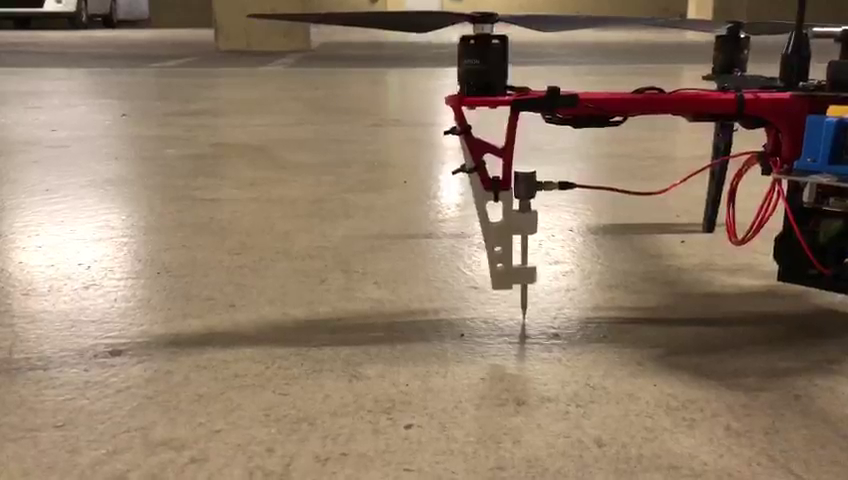
\includegraphics[width=5cm]{images/stage_graphs/vibration_results/measure_road.png}
    %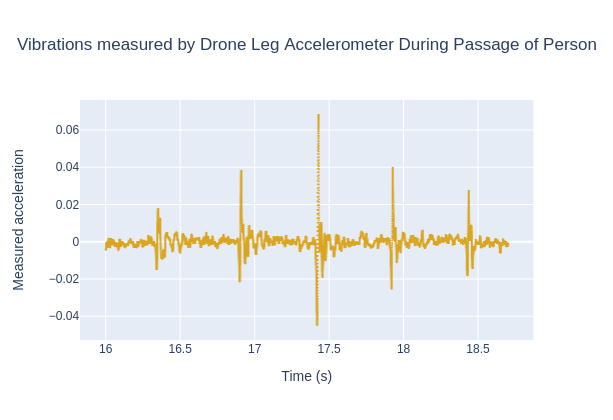
\includegraphics[width=9cm]{images/stage_graphs/vibration_results/footsteps.png}
    \caption{Footstep Detection with an Onboard Accelerometer}
    \label{fig:footstep_setup}
\end{marginfigure}

\textit{Detection of Footsteps with a Drone Vibration Solution}

% drone_vibration_why}
Structural inspections include seismic equipment upon UAVs \cite{stewart_chang_sudarchan_becker_huang_2016}, yet there lacks any mention of vibration probes on UAVs. We develop a drone prototype for acquiring vibration data after flying, landing, and recording under various scenarios (Figure \ref{fig:footstep_setup}).

% footstep_detection_evaluation}
We test the validity of a drone vibration solution by using real-world human walking experiments on a concrete floor structure. This approach is also taken in \citename{gait_analysis}{author} \cite{gait_analysis} (\citedate{gait_analysis}), who test an onboard UAV sensing module consisting of a series of geophones.


 %DRONE SENSITIVITY
\begin{marginfigure}%[!h]
    \raggedright
    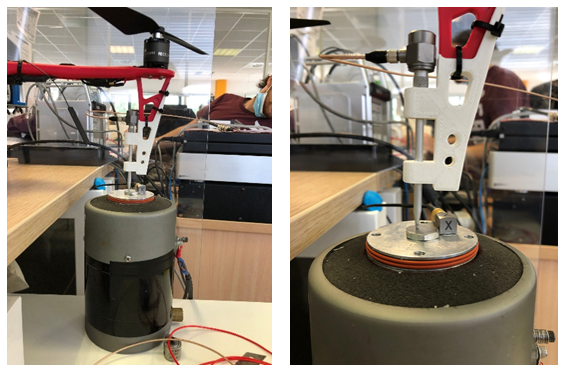
\includegraphics[width=5cm]{images/stage_graphs/vibration_results/vibration_test.png}
    \caption{Sensitivity Test: Experimental Setup}
\end{marginfigure}

\textit{Determining the Sensitivity of the Drone Vibration Solution}

% mount_sensitivity_evaluation}
We characterise the sensitivity of the drone probe solution with a sinusoidal sweep. A vibration shaker performs a sinusoidal sweep in a controlled setting.


\section{Overview of the Thesis}

\textbf{Chapter \ref{c1}: \nameref{c1}}

% c1_thesisgoal}
In line with the thesis goal, we seek to better understand how distributed systems can offer smart assistance to multi-robot development. We explore research and techniques designed to coordinate multiple robots.
% c1_contents}
We document the design of a development and demonstration testbed conform to existing research. We describe a procedural task-based architecture to complement an existing swarm stack. We demonstrate that the runtime environment is capable of coordinating multiple robots. A custom high level interface wraps the testbed towards more complex tasks, and it is demonstrated in a multi-drone choreography.

\textbf{Chapter \ref{c2}: \nameref{c2}}

% c2_thesisgoal}
In line with the thesis goal, we look at two types of smart systems that enhance the interactions between humans and drones. The first allows the human to pilot a drone through a gesture interface. The second looks to a virtual interface as a training ground for a real drone to avoid a virtual object. A distributed system is used to to communicate and coordinate these pipelines by passing messages to one another from any system. To better understand their tradeoffs, the distributed systems are explored and evaluated in this chapter.
% c2_contents}
We investigate a Mixed Reality Interface for the Testbed, as well as methods of drone Piloting using a Computer Vision algorithm. The utility of the framework is demonstrated by using it for two different tasks: quadrotor piloting using computer vision and collision-free flight of multiple UAVs. Building on existing frameworks like MediaPipe Hands, and Unity3D, we create perception pipelines for semi-autonomous flight, and we proceed to evaluate the response latency of these pipelines.

\textbf{Chapter \ref{c3}: \nameref{c3}}

% c3_thesisgoal}
In line with the thesis goal, we pay attention to the interplay between smart systems, and the real-world deployment of a UAV. The carrier drone aids in streamlining the data collection process, by automating different fly-by procedures, safeguards, and scheduling the data collection. Two payloads are tested in outdoor flight, for atmospheric data and vibration data, and the sensors used in these tests are evaluated. In this way, onboard systems can aid with the practitioner’s task.

% c3_contents}
Applications are explored for UAVs as Mobile Sensing Platforms, with high-sampling and high-precision equipment. We design a carrier drone and Onboard Data Acquisition systems and we put them to practice along standards defined by industrial practitioners. Two payloads are tested in outdoor flight, for atmospheric data and vibration data, and we characterise the sensors used for these tests. A vibration probe is designed and our tests demonstrate its relevance in the field of mobile sensing.
% \subsection{General Background}
% %\textbf{~0.5 pages}

% %\subsubsection{A. Concepts relating to Accurate Positioning}

%     \paragraph{\textbf{Control theory} }
%     Classical control theory is a field developed over the last century. It aims to drive the system to a desired state, while minimizing any delay, overshoot, or steady-state error and ensuring a level of control stability. This field was developed because basic localization in the real world is prone to error. Slight deviations in the instrumentation used to measure position, and influences from environmental factors, have it that a motor movement does not equate the desired motion.
    
%     % In control theory, the basic principle is to observe the motion of an object and grade specific information against the required motion. A setpoint is the desired or target value for an essential variable, or process value of a system. All feedback controllers are designed to eliminate discrepancies between the process variable and the setpoint.
    
% %\subsubsection{Concepts relating to Realtime Data Networking}

%     \paragraph{\textbf{A robot operating system}}

%     Developing a complete robotic system often requires combining multiple behaviours into a complex decision grid, with elements running in sequence or in parallel, eventually interrupting each other. The basic principle of a robot operating system is to run a great number of executables in parallel that need to be able to exchange data synchronously or asynchronously. For example, a robotics OS needs to query robot sensors at a set frequency (ultrasound, temperature sensor, gyroscope, accelerometer, cameras, microphone, etc.), retrieve this data, process it (carry out what is known as a data merge), pass it to processing algorithms (speech processing, artificial vision, SLAM – simultaneous localisation and mapping, etc.) and lastly control the motors in return. This whole process is carried out continuously and in parallel. Moreover, the robotics OS needs to manage contention to ensure efficient access to robot resources.

%     % The main idea of a robotics OS is to avoid continuously reinventing the wheel. This reduces development time, debugging, and testing effort, especially in safety critical devices where it needs to be shown that all possible risks and faults have been addressed and mitigated.
    
%     \paragraph{\textbf{Interoperability}}
%     %\color{ForestGreen} [What, why, how.] \color{black}
    
%     UAV flight has many simultaneous processes running in parallel: high level programs and low level programs, sensors and sensor monitors. Data can be exchanged synchronously or asynchronously between such processes. For instance, a sensor reading could be instrumental in the robot’s navigation. Most often, our robots must transmit information over wifi to a basestation. Such information can be used to issue commands to the robot remotely and assist the robot, but also can for observational purposes, to record data issued by the robot.

    
%     \paragraph{\textbf{Low-level device control}}
%     %\color{ForestGreen} [What, why, how.] \color{black}
    
%     Some UAV functionality is ensured via independent devices: power distribution to the motors, battery monitoring, or functionality operating on remote computers. We might want to exchange data synchronously or asynchronously with such devices. This is achieved via a robot operating system.

% %\subsubsection{Concepts relating to Smart Behaviours}
    
%     \paragraph{\textbf{Using Tasks for Defining Behaviours}}
    
%     %\color{ForestGreen} [What, why, how.] \color{black}
    
%     Autonomous UAVs sometimes need the development of automatic behaviours as tasks. One approach is to make each task start, run for some amount of time,  and then terminate either on completion or on interruption. Each tasks can be implemented programmatically as an Action. In this paper, tasks are therefore referred to as actions.
    
%     \paragraph{\textbf{Using a Central Server for Monitoring}}
%     %\color{ForestGreen} [What, why, how.] \color{black}

%     A central system may be involved in decision-making, especially as the network scales up to multiple agents. To affect the behaviour of each agent independently, it must be possible send different commands to separate agents. This is achieved programmatically through a Client-Server relationship, in the case of actions, an Action Server.
    
%     \paragraph{\textbf{Using a State Machine as the Client}}
    
%     A central system may choose between several decisions, by assessing the next decision from the state of each agent: 'going-to', 'landing', etc. In other words, the client requires ‘decision-maker’ between each state and a set of possible future states. It is possible to use a C++/python script to analyse camera information and to code up a sequence of actions. A \textbf{state machine} is a little more advance as it coordinates the transition between different usecases. Programmatically, the system will have a set of pre-loaded behaviours that can be instantiated by a State Machine, within the Client.
    
   
%     \paragraph{\textbf{Task Scheduling}}

%     A task manager is a system monitor program used to provide information about the processes and applications running on a computer. This definition can be extended to the UAV case, where it provides information on the state the drone is in: 'going-to', 'landing', etc. There are cases where the UAV processes are not only sequential but simultaneous, defined as \textbf{concurrence}. The processes are sometimes executed randomly and take precedence on the current task. This refers to \textbf{preemption}.
    
%     %\item \textcolor{red}{\textbf{Virtual Stigmergy}}



% \section{Motivation}

% There is a general consensus that intelligent robots might affect great change, but current UAVs have very limited swarm functionality. Several drones are commercially available, but their application scope remains limited to a single point-to-point link between a program and the drone, thus, it becomes time-consuming to develop applications for swarm research, for agile flight. Instead, these are active areas of drone research, championed bys dozens, even hundreds of drone laboratories.


% \section{Challenges}

% Any Parrot, or Astec UAV can be obtained on the market. However, beyond entertainment, it's difficult to see them as service robots.
% There is a general consensus that intelligent robots might affect great change, but current UAVs have very limited functionality.
% However, creating intelligent functionalities for UAVs is a challenging task.
% Where do we start with this development?

% \section{Scientific contributions}

% \begin{enumerate}
% \item As part of the testbed for service drones, we offer a library of well-known swarm behaviors, which is offered open-source to practitioners of the Crazyswarm Project.

% \item During outdoor deployment, we develop and characterise a vibration probe that showcases the advantages of high-precision and high-frequency in the field of Sensor Placement Research.
% \end{enumerate}